\section{Does Supervision Density Change Update Sparsity?}
\label{sec:density}

Broader vocabulary supervision can change the gradient at a prefix without proportionally increasing the number of parameters changed by the optimizer. Dense supervision and concentrated checkpoint changes coexist in the experiments of \citet{yu2026denseupdates}. We examine this relationship through a local comparison at a common state and online PG/I64 comparisons in single-teacher and joint training.

\subsection{Comparison and measurements}

PG uses the sampled-token loss in Equation~\ref{eq:pg}. I64 scores the intersection of the rollout student's and teacher's top-64 sets, with detached student weights normalized over the original student set. Its formula appears in Appendix~\ref{app:losses}. The online configurations are S-PG and S-I64 with the mathematics teacher, and M-PG and M-I64-DR with four routed teachers. Within each setting, the branches share initialization, teachers, domain-response averaging, optimizer settings, and prompt schedule. The single-teacher branches use 64 mathematics responses per update; joint branches use 16 per domain. We compare PG and I64 within each setting at common checkpoints.

The local experiment evaluates PG, I64, corrected teacher-top-64 supervision (T64), and full-vocabulary reverse KL on the same four prefix banks at M-PG update 100. Each bank contains one response per domain and six selected prefixes per response, for 16 responses and 96 prefixes in total. Responses use the training cap of 4,096 tokens; two responses reach the cap. Every loss uses identical prefix weights and the same saved optimizer state. We compute the fraction of changed parameters and the fraction of squared step norm carried by the largest 1\% of coordinates.

\subsection{Update concentration}

\paragraph{Local changes are similarly concentrated across losses.}
Figure~\ref{fig:density} shows that all four losses change about 88.0\% of FP32 coordinates. Mean BF16 nonzero fractions are 0.149\% for PG and 0.150\% for I64, T64, and full vocabulary. The largest 1\% of coordinates carry about 8.8\% of the FP32 squared step norm and all of the BF16 squared step norm. Local concentration is therefore very similar across the four losses at this shared state. The shared Adam history contributes to this result: a zero-current-gradient control alone changes 0.140\% of BF16 coordinates.

\begin{figure}[t]
\centering
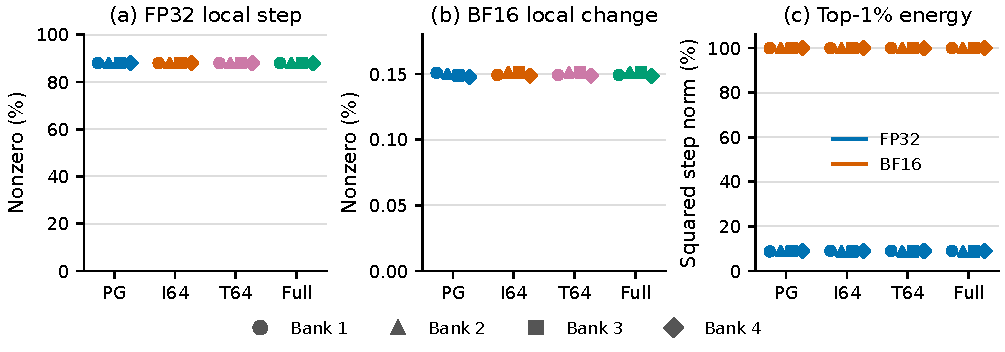
\includegraphics[width=\linewidth]{figures/aligned_evidence_20260910/supervision_density.pdf}
\caption{Local supervision comparison at M-PG update 100. (a,b) Nonzero fractions for FP32 optimizer steps and BF16 model changes. (c) Squared step norm in the largest 1\% of coordinates. Points show four prefix banks; every loss uses the same saved optimizer state.}
\label{fig:density}
\end{figure}

The teacher's top-64 tokens contain a mean 99.918\% of student probability across these prefixes, with a minimum of 96.709\% at an individual prefix. The selected vocabulary therefore retains most of the student probability in this experiment. Appendix~\ref{app:losses} gives the sampling and coverage details; Appendix~\ref{app:records} provides separate threshold and optimizer-state controls.

\paragraph{Joint trajectories accumulate different changes.}
Figure~\ref{fig:geometry} compares cumulative PG and I64 changes under the same joint training protocol. At update 250, I64 changes 7.13\% of BF16 coordinates versus 5.88\% for PG; the coordinate fractions accounting for 90\% of squared change are 3.94\% and 3.01\%. Broader vocabulary supervision therefore accompanies broader cumulative activity in this comparison, while both remain concentrated. The local experiment fixes the student, prefixes, and optimizer state; the online comparison includes the feedback between each loss and the responses its student generates.

\subsection{Capability under single-teacher and joint training}

Table~\ref{tab:density_capability} reports PG/I64 pairs: updates 100, 250, and 500 for the single-teacher branches and 50, 100, and 250 for the joint branches. In single-teacher training, PG's mathematics score exceeds I64 by 2.8 points at update 100, whereas I64 exceeds PG by 2.2 points at update 500. At update 500, I64 also scores 0.67 points higher on instruction following, while PG scores 1.56 points higher on code and 1.77 points higher on GPQA.

In joint training, both losses reach 26.0\% on instruction following at update 250. I64 reaches 74.8\% on mathematics, 17.97\% on code, and 33.96\% on GPQA, compared with PG's 73.4\%, 16.41\%, and 30.18\%. The I64-minus-PG GPQA difference is 3.79 points, with a paired prompt-bootstrap interval of $[0.00,7.58]$. Its four-domain mean is 38.18\%, compared with 36.50\% for PG. These endpoint scores favor I64 in the joint setting, while the single-teacher comparison retains domain tradeoffs. Figure~\ref{fig:capability} shows all matched trajectories, and Table~\ref{tab:endpoint_paired} gives all eight endpoint differences with their paired intervals.

\begin{table}[t]
\caption{Online PG/I64 capability pairs (\%). Each pair shares the setting and update count. Mean averages the four domain scores. Single-teacher and joint updates have different per-domain response counts.}
\label{tab:density_capability}
\centering\small
\begin{tabular}{lrrrrrr}
\toprule
Configuration & Updates & Math & Code & IF & GPQA & Mean \\
\midrule
S-PG & 100 & 77.40 & 18.75 & 18.67 & 31.82 & 36.66 \\
S-I64 & 100 & 74.60 & 18.75 & 17.67 & 33.21 & 36.06 \\
S-PG & 250 & 73.80 & 20.31 & 17.00 & 35.35 & 36.62 \\
S-I64 & 250 & 74.40 & 21.09 & 18.33 & 32.45 & 36.57 \\
M-PG & 50 & 69.60 & 16.41 & 18.67 & 28.03 & 33.18 \\
M-I64-DR & 50 & 69.60 & 17.19 & 19.00 & 31.69 & 34.37 \\
M-PG & 100 & 72.00 & 17.19 & 19.33 & 31.19 & 34.93 \\
M-I64-DR & 100 & 71.60 & 17.97 & 19.00 & 32.70 & 35.32 \\
\bottomrule
\end{tabular}

\end{table}

The capability comparison and the local update comparison answer different parts of the supervision question. Broader feedback yields almost unchanged concentration at the fixed state, but the trained students develop different capability profiles. The matching single-teacher parameter measurements are specified in the annotation in Section~\ref{sec:subnetworks}.
